\documentclass{ltjbook}
\usepackage{docmute}
\usepackage{../../myStyle}

\begin{document}
\VerbatimFootnotes

\chapter{ベイズで判断する}
\label{ch27_bayes_judgement}

心理学において，ベイズ法は比較的新しく導入されたものです。
これまでは，後期から学んでいるように，要因計画と帰無仮説検定を組み合わせることで，群平均の差があるかどうかの判断を心理学理論の検証に使ってきていたのでした。では，新しくベイズ法が導入されることで，この帰無仮説検定はどのように変わるのでしょうか。ここでは，ベイズ法を使った判断の仕方について，心理学の研究における帰無仮説検定との違いを中心に説明していきます。

先に確認しておくと，帰無仮説検定はモーメント法，つまり母数がある値であるという前提のもとで標本から推論する立場でした。
これに対してベイズ法は，母数が確率的なもの，確率分布として推論する立場という，考え方の転換があるわけです。このことは，推論に基づく判断に大きな影響を与えます。すなわち，モーメント法・頻度主義の立場では，母数に「差があるか・ないか」は必ずどちらかひとつです。真実はいつも一つ。だからこそ，「母数に差がある時に，間違って標本から差がないと判断してしまう場合」といった，タイプ1エラー，タイプ2エラーという考え方が出てきたわけです。これに対して，ベイズの立場では差が「ある」「ない」のような固定的な状態ではなくて，「差の大きさ」という確率分布として出てくることになります。真実はいつも分布。であれば，タイプ1エラー，タイプ2エラーという考え方そのものがなくなります。その他，帰無仮説検定を実践する上での注意点(第\ref{ch14_NHST2}講)で触れたようなことも，ほとんどその前提から変わってしまうので，該当しなくなってしまうのです。なんということでしょう。

このことを念頭に置いて，それではベイズ法による判断のロジックをみていくことにしましょう。

\section{ベイズ法と帰無仮説検定}

\subsection{帰無仮説検定の考え方を振り返る}
ベイズ法での判断の違いをみるために，改めて，\keyterm{帰無仮説検定}{きむかせつけんてい}{null hypothesis significance testing}の考え方をもう一度振り返っておきましょうか。

まずさまざまな個人差や誤差が含まれるであろうデータに対して2つのグループを作って(多群でもいいですが)平均化し，そのことで個体差を相殺，一方の群にのみ影響があるような操作を行なって，結果の群平均を見ることで，平均的な\keyterm{因果効果}{いんがこうか}{causal effect}を見ることができるという\keyterm{要因計画}{よういんけいかく}{factor design}を使って研究が行われます。この要因計画は，影響源をさまざまな要因と交互作用に分解していく\keyterm{線形モデル}{せんけいもでる}{linear model}であり\footnote{分解していくというのは，全体の変動を要素の足し算に分解していくという意味です。単純な足し算にしているので線形(一次関数)モデルです。}，これを使って効果の大きさを見ることができるのでした。

ただ標本の効果の大きさだけでは限界があるので，これを\keyterm{母集団}{ぼしゅうだん}{population}の世界での話に広げたい。そこで\textbf{推測統計学}の出番です。平均値の位置や効果の大きさを，標本から推定していくわけです。

帰無仮説検定ではさらに，効果があったかなかったかという判断を行うための基準を用意してくれたのでした。効果がないというモデルvs効果がなくはないという2つの仮説＝モデルを立てて，どちらのモデルが良いものかを検討します。

その際，いったん効果がないというモデル(=\keyterm{帰無仮説}{きむかせつ}{null hypothesis})の立場に立って，効果がないと仮定した上でのモデル上の計算を進め，実現値がそのモデルからどれぐらい逸脱しているのかを考えるのでした。ここで効果が誤差に比べてどれぐらい大きいかという，分散の比の分布($F$分布)を用いたり，二群の平均の差の分布(t分布)を用いたりして，実現値がどれぐらいあり得ないかを考えます。これが事前に決めた判定基準，すなわち\keyterm{有意水準}{ゆういすいじゅん}{significance level}よりも小さければ，滅多にないことが現実に生じているわけですから，帰無仮説が間違っていたのだ，と考えるのです。ここで，帰無仮説が間違っていたのだとなると，「差がないとは言えない」という結論になります。その結論を使って「もう少し検討しないとな」と考えるもよし，「差がないとは言えないというのは，差があるということだな」と判断するもよし，です。後者の場合は「本当は差がないのに差があると言ってしまう間違い(\keyterm{タイプ1エラー}{たいぷ1えらー}{type I error})」とか，「本当は差があるのに差がないと言ってしまう間違い(\keyterm{タイプ2エラー}{たいぷ2えらー}{type II error})」が生じる可能性があるので，注意しなければなりません。差があるかないか，という判断に飛びつくのではなく，どれほど効果があるのか量的に判断すべきで，この効果の大きさについては\keyterm{効果量}{こうかりょう}{effect size}という指標を使って報告する，というフォーマットがあるのでした。また，判断を繰り返しすぎると，タイプ1エラーがコントロールできなくなりますから，分析は慎重に，まず\keyterm{主効果}{しゅこうか}{main effect}をみてから事後の検定へ，といった丁寧な進め方をしなければなりません。

ふう！ここ何コマもかけて説明してきたことを，1つのパラグラフにまとめるとこんな感じになります。十分面倒ですね！とくに「差がないとは言えない」とか，「差があるのにないと言ってしまう確率」のあたりで頭が混乱してくるのではないでしょうか。少なくとも私はいつも，教えていながら間違ってやしないか，ヒヤヒヤしております。どうしてこんなややこしい方法がありがたがられるのでしょう？それはひとえに，この考え方でいくと，出てきたデータが正規分布から得られていそうだということさえ仮定できれば，機械的にこの検定手続きを進めていくことができるからです。
\subsection{帰無仮説検定のありがたさ}
帰無仮説検定の話は，農学からでてきました。農業試験場で作物の成長についての実験をしていたところから，区画を分割して効果を比較するといったアイデアが形になっていったわけです。しかし一度，この分析のフォーマットが出来上がると，心理学でも利用できますよね。人間は農業試験場で取れる生産物ではありませんが，さまざまな特徴は正規分布してそうなので，利用すればいいのです。別に心理学に限りません。生物学でも，経済学でも，物理学でも，社会学でも，なんでも結構です。データが分布するとか，誤差が正規分布するといったアイデアがあれば，応用は可能です。しかもこの分析手続に含まれる，面倒な計算！とくに$t$分布がどうだとか，$F$分布がどうだとかいうことを数理的に導出しようとするととても大変ですが，計算のフォーマットは定まっているわけですから，Rの関数にポンといれれば結果を出してくれる。難しいことを考えなくても，結果は出てくるのです。これが帰無仮説検定がありがたい理由で，フォーマットが定まっているからさまざまな領域に応用できること，その計算フォーマットを実装した統計パッケージが利用できること，これが大きいのです。

これのおかげで，必ずしも数学が得意ではないわたしたち心理学徒でも，統計の力を借りることができるようになりました\footnote{しかしこのことが問題にもなってきています。すなわち，よくわかってないのに使って，結果だけ見て考えるというようなことが起こってしまうわけです。免許も持っていないのに，とりあえずアクセルを踏んだら車が走るから踏んでみた，というような話ですね。そんな怖いことを現実社会でやったらとんでもないことなのですが，でも統計の話って難しいし，専門的すぎてどこかは機械や先人に任せるしかない。車だって，MT車じゃなくてAT車のほうが普及していますし，素人がAT車のコンピュータ制御部分を修理したりできるほど専門知識を持ってるはずないですもんね。全部わからないと運転してはいけない，というのはちょっとやりすぎです。つまり私たちは，免許を持てる程度に基本的な知識を身につけ，悪用・誤用をしてしまわないように気をつけなければいけないのです。また，免許には更新があるように，統計の勉強を普段から怠っていてはいけません。新しい技術が使いこなせないと思った場合は，免許返納・車に乗らないという判断もするべきです。}。

私たちは心理学が専門ですから，統計のことはよくわからない，ツールをつかうユーザの立場でしかない。というのはその通りだと思います。しかし同時に，心理学が専門だというのであれば，その結果の解釈や意味の理解にこそ，もっと責任を持たなければなりません。先ほど帰無仮説が棄却された場合について言及しましたが，差がないと言えるかどうか，判断基準を機械的に決めるのは確かに1つの方法です。しかしその前に，どの程度の差が実質的な意味を持つのか，何をもって差があると言えるのかについて，丁寧に考える必要があるでしょう。帰無仮説検定はあくまでも，区間推定の結果を判定するやり方の1つであり，そもそも推定された平均値の差，その区間，効果量や効果量の信頼区間について，考える必要があるのです。

ここで注意が必要なのは，従来の頻度主義的な考え方では，推定される平均値は定数として定まったものであるということです。\keyterm{信頼区間}{しんらいくかん}{confidence interval}は，その区間の中に推定された平均値が\textbf{含まれる割合}，\textbf{正答率}を示す数字であり，区間と言いながら幅の情報を持っていない幅なのです。これに対して，ベイズ法での推定値，たとえば群ごとの平均値の事後分布から考えられる\keyterm{確信区間}{かくしんくかん}{credible interval}は，確率的に分布する平均値の\textbf{とりうる範囲}を示す数字であり，幅の情報そのものです。ベイズ法で推定される平均値の区間推定は，下限から上限の範囲に含まれる領域，あるいはあると思われる信念の領域を表しており，当たり外れの問題ではないのです。

\subsection{ベイズ法のありがたさ}
ところで，ベイズの考え方は事前分布を必要とします。これについては，「分析の前に差があるだろうとかないだろうとか，主観的な思い込みを持ってデータを弄るのはケシカラン」という批判がなされることもあります。しかし逆に，何の前提も置かないことが，果たして良いことなのかどうか，という話もあるのです\parencite{Maeda2017}。

たとえばコイントスをして「24回投げて7回は表が出た」話があったとしましょう。これは公平なコインか，というのを帰無仮説検定したいと思います。帰無仮説はコインが表になるか裏になるかに偏りはない，というもの。対立仮説は何らかの偏りがある，というものです。データは半分(12回)を少し下回っていますから，ちょっと怪しいところではありますが，実際に帰無仮説検定をするとこれは帰無仮説を棄却できません\footnote{表7，裏14という度数分布に偏りがあるかどうかは，$\chi^2$検定(カイにじょうけんてい)を使います。Rで\texttt{chisq.test(c(7,14))}と書くと，統計量$\chi^2(1)=2.33,p=0.1266$という答えが得られます。}。つまり，7/24という結果は5\%よりも生じやすい結果であり，驚くほどのことではないということになります。

しかし，この例がコインではなくて釘だったらどうでしょう？ 釘をトスして，頭の部分が底になって地面の上にピンと立ち上がったら表，そうでなかったら裏だと考えるのです。それで，24試行中7回ピンと立ち上がったとします。なんで？ おかしくない？ 珍しくない？ すごくない？

こんな時でも，帰無仮説検定は棄却できません。24回中7回表が出た，という事実は事実ですから，「おかしくない。こういうことだってある」という結論になります。私たちが「そんな馬鹿な，地面に磁石でもあるんだろ」などと思うのは，放り投げた釘が立ち上がることなんてあり得るはずがない，と強い信念を持っているからです。その信念は物理的な法則に裏付けられたものであり，十分に納得のいくものでしょう。しかしこうした信念すら「事前の思い込みはいけない」といって無視し，「事前に何も思い込みを持ってはいけない，出てきたデータがすべてだ」という態度を取るのであれば，偏りがあるとは言えない，という答えを支持するしかありません。これが科学者の定めでしょうか？

これは，コインや釘といった違いを無視して，「表か裏か」という度数だけにしてしまったところに問題があります。データが得られるメカニズムは全く無視して，その表面的な度数だけ数えて考えています。事前情報を無視して(あるいは明記せずに)，結果だけで判断するのは，かえってフェアな態度ではないというべきです。これに対してベイズ推定をする時は，事前分布と尤度を明記しなければいけません。事前分布は研究者の事前知識を，尤度はデータが出てくるメカニズムを表しています。表か裏か，という結果もどういうメカニズムから2値になったのかを書き込むことができます。これを明確に記録するベイズ統計のほうがより開かれた態度だということもできるでしょう。

\section{確信区間に基づく判断}
\subsection{確信区間の解釈}
帰無仮説検定が面倒になる一番の理由は，判断が確率的になることです。判断して間違える確率，というところまで考えないといけないのでややこしいですね。
これに対して\keyterm{ベイズ法}{べいずほう}{Bayesian method}は，「正しい世界」「間違えた世界」を考えるわけではなく，「私が信じられる世界」を考えるので，こうした面倒が生じません。

例として，一要因3水準群間デザインをとりあげ，これをベイズ推定したとしましょう。このデザインは第\ref{ch17_RCT}講でもやったもので，3つの群から推定される母平均が同じかどうかということが問題になるのでした。何にせよ正規分布を仮定していますから，3つの群A,B,Cについての確率モデルは，
\[ X_{i1} \sim N(\mu_A, \sigma), X_{i2} \sim N(\mu_B, \sigma), X_{i3} \sim N(\mu_C, \sigma)\]
となっている，と書くことができます。ここで$X_{ij}$は，$j$群に属する$i$さんのデータ，という意味であり，対応関係がないのでそれぞれ異なる3つの平均値$\mu_A,\mu_B,\mu_C$の正規分布から出てきているということをこの式が表しています。分散分析の時は，母分散が均等であるという仮定をおきますから，$\sigma$には群わけの添字がありません。

これをベイズ推定して，それぞれの群の平均値が得られたとしましょう。結果を図\ref{fig:27_05}に，各群の平均値の推定結果とその95\%区間とともに示しました。この結果から「差があるかどうか」という意思決定をどのようにすれば良いでしょうか。
\begin{figure}[ht]
	\centering
	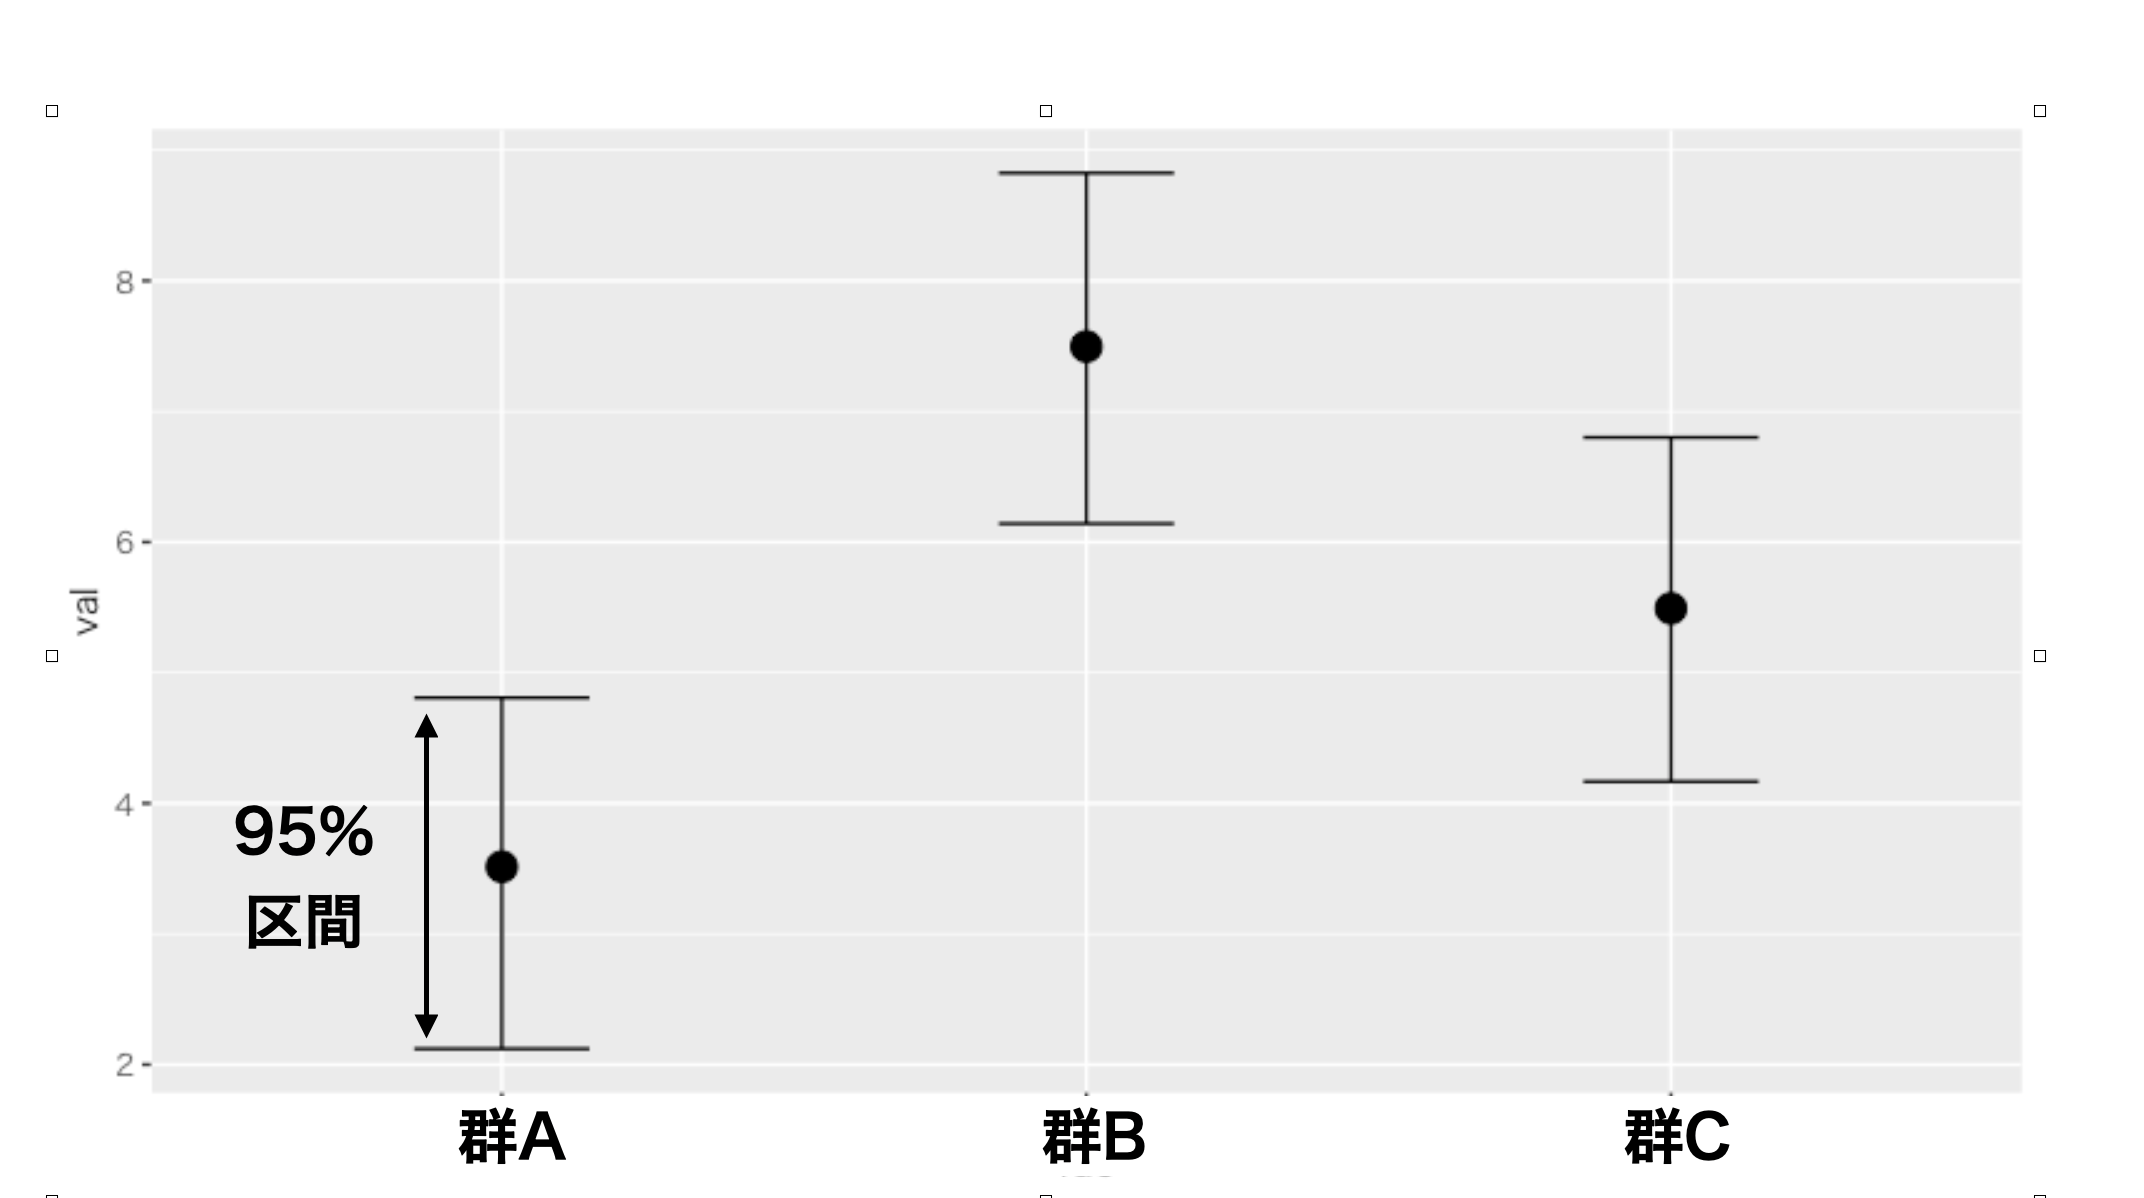
\includegraphics[keepaspectratio,width=0.8\linewidth]{figures/27_bayes_judgement/BayesianJudgement.png}
	\caption{ベイズ推定による推定結果}
	\label{fig:27_05}
\end{figure}

意思決定に際して，帰無仮説検定は「帰無仮説と対立仮説というモデル対決」に持ち込んでいき，5\%の判定ミスを許容した上で決断するのでした。どうしてこのような形になっているかというと，母平均はどこか一点にあって，われわれはそれを探っているから，究極的には推定が「あっているか間違っているか」の2択にしかならないからです。

ところがベイズ主義的には，母平均はどこにあるのかわかりません。わからないので「この辺りにありそうだ」というのを確率で表現しています。それは知り得ない1点があるのか，それともそもそも確率分布としてあるのかは，哲学的観点が分かれるところです。何にせよあるかないか，という点の勝負ではなく，そもそも分布の勝負になっているので，この95\%区間のどこかにあるとだけしておきましょう。図には95\%区間を描いていますが，この幅のどこかに存在するとしたら，群Aの上側95\%点よりも群Bの下側95\%点の方が上にあって，この両群の確信区間は重複する領域がありませんから，この2群ははっきりと差がある，ということができます。一方，群Aと群C，群Bと群Cは区間に重複がありますから，これらの組み合わせは差があるとは断言できない，ということになります。

That's all!これで終わりです。帰無仮説検定の場合は差があったとしても「差がないとは言えないし，そういってしまって間違える可能性が5\%」というのが正しい表現でした。まだるっこしいですね。これに対してベイズ推定した結果は，「95\%の確信度で差がある」ということができます。ここでいう確信度とは言葉の通りこの主張の強さを表していますから，50\%でも99\%でも構いませんし，95\%よりも99\%の方が確信度が高い，つまりより強く主張していることになります。帰無仮説検定の時の$p$値についてはこのような判断ができなかったのに比べて，非常に直感的でわかりやすい結果になっています。$p$値については，5\%と1\% を比べて1\%のほうが強い，などと言えないのでした。それは$p$値がデータや母数についての数値ではなく，1.帰無仮説という仮定を置いた上での，2.現実値の珍しさの度合いを表す，3.判定基準にすぎない，というものだったのでした。これに比べるとベイズ推定して得られた結果は，1.母数の推定された区間，これだけですので，推定値で物事を考えるのにもってこいです。こうなってくると，5\%にこだわった考え方が無意味であることが一層はっきりしてきますね。

この話は，ベイズ法でなくても別にいい話ではあります。というのも，頻度主義的なモーメント法による区間推定で，信頼区間をみて「差があるかなあ，ないかなあ」と考えることはできたわけです。どの群の信頼区間も大きくて，群間のそれが重複しているようであれば，平均値がどのあたりにありそうなのかわかりにくいわけですから，判断するには時期尚早。信頼区間が小さければ，判断があたるか外れるかのチェックをしてもいいけど，という感じで利用することもできます。何が言いたいかというと，帰無仮説検定は「判断」を定めることに無理があったのであり，科学的な研究アプローチとしては「外れたから研究は失敗」という短絡的なものではなく，徐々に何が正しいのかに近づいていけさえすれば良いのです。\textcite{Toyoda2009}が指摘するように，重要なのは\textbf{有意差}ではありません。むしろ重要度はそれが一番小さくて，
\[ \mbox{有意差} < \mbox{標準化された差(効果量)} < \mbox{実質的な差} \]
の順に意味があるのです。データが実質的にどれぐらい違うのか，標準偏差いくつ分ぐらい違うのか，ということが大事なのであって，判断結果で有意差があるかどうかは大したことではありません。
\subsection{実質的に等価な範囲による判断}
とはいえ，確信区間や信頼区間を見て「差があるかなあ，ないかなあ」と思いを馳せるだけでは，レポートには書きにくいですね。そこで事前に，どれぐらいの差があれば良いと判断するかという基準を決めておく，というのがいいかもしれません。
\textcite{kruschke2018rejecting}は，\keyterm{実質的に等価な範囲}{じっしつてきにとうかなはんい}{region of practical equivalence, ROPE}という幅を事前に定め，そこに(差の)事後分布の\keyterm{最高密度区間}{さいこうみつどくかん}{highest density interval}がどの程度含まれるかで判断すべきである，という主張をしています(図\ref{fig:27_04})。

\begin{figure}[ht]
	\centering
	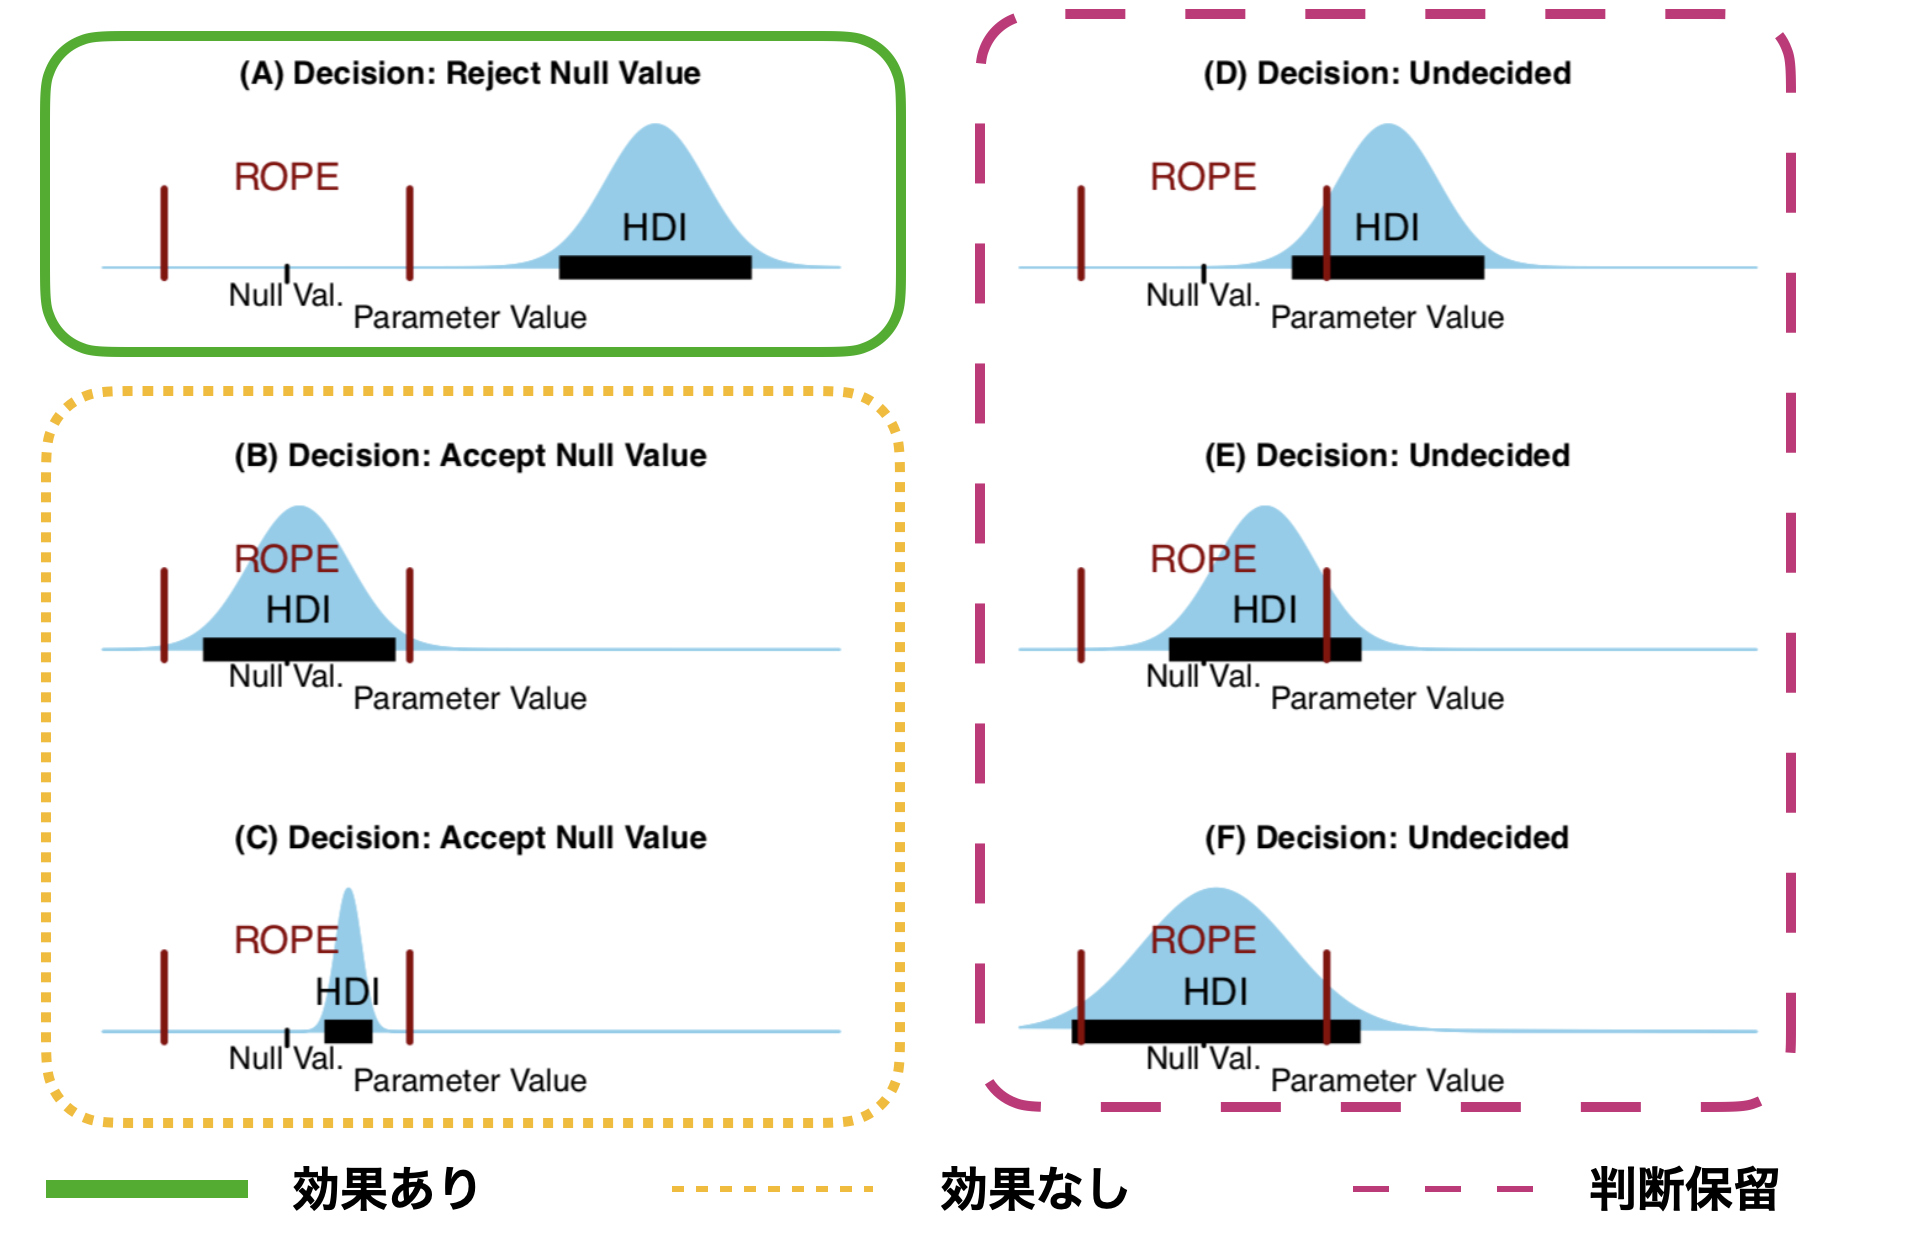
\includegraphics[keepaspectratio,width=0.8\linewidth]{figures/27_bayes_judgement/Krschke2018.png}
	\caption{実質的に等価な範囲による判断\parencite{kruschke2018rejecting}}
	\label{fig:27_04}
\end{figure}

ROPEを使った判断をするためには，まずROPEを決める必要があります。それをどうやって決めるんだ，ということについてまた議論があるかもしれませんが，それは分析を応用する各領域において，その領域専門の知識(ドメイン知識)に依存する話なので一般論として語ることはできません。たとえば数字の上で1ポイント差があるというのが，男女の平均身長差の話であれば(そして単位がcmであれば)，なんだ1cmの違いなんか実質的に意味ないね，という話になるでしょう。しかし1人の女性が一生のあいだに産む子どもの数(合計特殊出生率)の国際比較であれば，子供が1人多いか少ないかというのは結構重要な差になります。錯視量が1cmなのは大きいでしょうか？ 回転角が1度ちがうのは？ 反応時間が1ms違うのは？ こうした話はいずれも，単位とドメイン知識に依存することなので，一律に言えないのです。帰無仮説検定は一律に5\%と言ってくれました。しかしそのことが，大事な何かを見失わせたのかもしれません。ここを手抜きせず，しっかり考えることが第一歩です。

仮に，ROPEを$[-1.0, +1.0]$と定めたとしましょう。ROPEは実質的に等価＝差がない範囲ですから，今回$0$を挟んでいます。さてベイズ法の場合，データから得られる平均値の差というのも事後分布として，幅を持ってえられます。例えばこの差$\delta$の事後分布の95\%HDI区間が，$[+1.5, +3.0]$であったとしましょう。これはROPEの範囲外です。図\ref{fig:27_04}の(A)のように，完全に外れていますから，これは差があると判断していいでしょう。逆に図の$B$の上のように，95\%HDI区間が$[-0.5, +0.5]$の場合。完全にROPEの中に含まれていますから，これは実質的に等価。差があるとは言えません。仮にこの95\%HDI
区間が短く，$[+0.4, +0.6]$のように$0$を跨いでいなくても，ROPEの中に入っている場合はやはり，差があるとは判断しません。そして図の右にあるように，(上)HDI区間が$[+0.5, +1.5]$のように，ROPEに一部引っかかっている場合，(中)HDI区間が$[-0.3, +1.3]$のように一部はみ出したけれどもROPEの中に入っている場合，(下)HDI区間が$[-1.2, +1.2]$のようにROPEをよりも広い場合。これらはいずれも「判断保留」とするのです。上・中はどちらの可能性も含まれていますし，下の図はHDIが広くて証拠不十分，というわけですね。「結局差があるかないか，どっちなんだ」という判断には時期尚早で，科学的な態度としては拙速な判断の方が弊害が大きいので，正直に「まだそこまで言える状態ではないですよ」というのが正しい態度です。

ベイズによる判断は，確率分布を使うからはっきりしない，と思うかもしれませんが，急いではっきりさせられるほど心理学の事象は明確でもないし，心理学の理論は強固でもないのです。だからこそ，確率分布を使って，まだそこまで言えない，ということを正直に表明するのが科学的な態度ではないでしょうか。

\section{ベイズファクター}
ベイズを使った判断基準について，もう1つ別の角度から紹介しておきましょう。それが\keyterm{ベイズファクター}{べいずふぁくたー}{Bayes factor}です。

もう一度ベイズの公式を見てみましょう。ベイズの公式は次のようなものでした。

\[ p(\theta\mid D) = \frac{p(D\mid \theta)p(\theta)}{p(D)} \]

言葉で言うと，事後確率は事前確率と尤度の積を\keyterm{周辺尤度}{しゅうへんゆうど}{marginal likelihood}で割ったもの，となります。
ここまで事後分布の形に注目してきたため，分子に当たる事前確率と尤度の方に話が集中していましたが，ここでは分母に目を向けます。分母は$p(D)$，つまりデータが出てくる確率で，定数なので考えなくていいよと言う話をしてきましたが，モデル比較ということを考えると，重要な意味を持ってきます。

さて帰無仮説検定は，帰無仮説というモデルと対立仮説というモデルの対決だ，という話をしました。あるモデル$\mathcal{M}$をつかって検証する，という条件をこのベイズの公式に追加してみましょう。

\[ p(\theta \mid D,\mathcal{M}) = \frac{p(D\mid \theta,\mathcal{M})p(\theta \mid \mathcal{M})}{p(D\mid \mathcal{M})} \]

すべての要素に「あるモデルという条件のもとで」という条件が追加されています。今度はここで分母に注目します。分母の$p(D\mid \mathcal{M})$を言葉にするならば，モデル$\mathcal{M}$が与えられた時のデータの確率，ということになりますね。
ここでモデル$\mathcal{M}$はパラメータ$\theta$を持つモデルなのですが，このパラメータがかりに2つしか状態を持たない，たとえば$\theta_1$と$\theta_2$しかないのであれば，この2つを使って次の計算ができます。

\[ p(D\mid \mathcal{M}) = p(D\mid \theta_1,\mathcal{M})p(\theta_1\mid \mathcal{M}) + p(D\mid \theta_2,\mathcal{M})p(\theta_2\mid \mathcal{M}) \]

これはつまり，$\theta$で\keyterm{周辺化}{しゅうへんか}{marginalization}したことになります。確率のすべてのパターンを足し合わせると，そのパラメータが消えてしまうわけですね。K個の状態を保つ離散的なパラメータの場合に一般化して書くと，次のようになります。

\[ p(D\mid \mathcal{M}) = \sum_{k=1}^K p(D\mid \theta_k,\mathcal{M})p(\theta_k\mid \mathcal{M}) \]

連続的なパラメータであっても，総和$\sum$の記号が積分記号$\int$に変わるだけで，式としてはほぼ同じです。

\[ p(D \mid \mathcal{M}) = \int p(D\mid \theta,\mathcal{M})p(\theta\mid\mathcal{M}) d\theta \]

さてこのように考えると，$p(D \mid \mathcal{M})$はモデルを考えた上でのデータが得られる確率，ということであり，求め方は「モデルが想定するすべての確率を網羅的に数え上げたもの」ということになります。
検定のロジックは帰無仮説と対立仮説という2つのモデルでしたから，$p(D \mid \mathcal{M}_{null})$と$p(D \mid \mathcal{M}_{alt})$というモデルを比較するという話だったことになります。
そしてこの確率は，想定したモデルからデータが得られる確率，という意味ですから，言い換えると\underline{想定したモデルがどれほどデータに支持されているか}ということでもあります。モデルの想定通りのデータが出てきたのであれば，この数字は大きな値になりますし，モデルの想定していなかったデータが出てきたのであれば，この数字は小さくなります。もしモデルが「どんなデータでも出てくるよ」というような漠然とした広ーい予測しかしていなかった場合，これはパラメータの範囲がごく広いということですから，そのごく広い範囲すべての場合にわたってデータを計算すると，相対的に予測していないところからデータが出てきていることが多くなり，結局この値は小さくなります。つまり「なんでも説明できるモデル」は何も説明しないことになるのです。この値が，モデルがデータに支持されている程度を表している，ということの意味が伝わりましたでしょうか。

その上で，次のような数字を考えます。

\[ BF_{12} = \frac{p(D\mid \mathcal{M}_1)}{p(D\mid \mathcal{M}_2)} \]

この数字は\keyterm{ベイズファクター}{べいずふぁくたー}{Bayes factor}と呼ばれるもので，モデル2に比べモデル1がどれほどデータに支持されているかを示す数字です。この数字が1.0より大きければ，モデル1はモデル2に比べて相対的に強くデータに支持されているということになります。逆に1.0を下回ると，モデル2のほうがモデル1よりもいいね，ということです。モデル同士の比による表現ですので，$BF_{21}$としても構いません。ここでモデル1が対立仮説，モデル2が帰無仮説だとすると，どちらがよりデータをうまく表しているか，どちらがよりデータに支持されているかがわかるわけですが，このやりかただと「差がない」という帰無仮説を積極的に支持することもできます。このように指標化されると，私たちはつい「じゃあBFがどれぐらいの大きさだったらいいんだ」と目安を求めてしまいがちですが(そしてそれは一般に3以上と言われていますが)，$p$値の5\%を目指した研究が陥ったのと同じ無意味な目標数値になってしまうかもしれませんので，そういうことは考えない方が良いかもしれません。

ともかく，これがベイズ流のモデル比較の方法のひとつです。他にも情報量統計学の観点からモデルの予測力などで評価する方法\footnote{WAICという指標を使います。詳しくは\textcite{Hamada201912}などを参照してください。}などもありますが，いずれもこの周辺尤度を使うやり方です。問題は，この周辺尤度の計算がとても難しいということにあります。パラメータが複数になると，分母のところにあらゆるパラメータのあらゆる組み合わせについて，重積分をしないといけないことになります。これは数値計算上とても難しいことで，実用面ではなかなか厳しいというのが本当のところです。

しかし，帰無仮説と対立仮説という関係なら，簡便的にベイズファクターを算出する方法があります。たとえば二群の平均値の差の検定に関して言えば，帰無仮説は$\mu_1=\mu_2$であり，対立仮説は$\mu_1 \neq \mu_2$というものでした。対立仮説は2つの母平均がイコールでなければすべてOK，という仮説であり，言い換えれば$\mu_1-\mu_2\neq 0$ということです。つまり差である$\mu_1-\mu_2$をX軸に取ったとすると，帰無仮説は$X=0$というピンポイントな，ごく部分的な仮説になっています。対立仮説の広い範囲の中で，帰無仮説はその一部・特殊ケースということであり，このようにネストされた仮説の場合は\keyterm{サヴェージ・ディッキー法}{さゔぇーじ・でぃっきーほう}{Savage-Dickey method}\parencite{Lee201709}という計算法でベイズファクターが計算できることがわかっています。

\section{ベイズ法による判断のひろがり}
% 移設元: ch27_bayes_judgement.old  L206--206「ベイズ法による判断のひろがり」

\subsection{ベイズ推定の利点}
% 移設元: ch27_bayes_judgement.old  L207--226「ベイズ推定の利点」
% シラバスb27に合わせ，以下の3点を柱に整理する
%   (1) 効果をそのままの大きさで語れる
%   (2) 多重比較のような補正がいらない
%   (3) 帰無仮説を積極的に支持できる

% 「生成量による新しい仮説の立て方」は ch29 へ移設（元: L227--248）
% 「ベイズの世界の広がり」は ch30 へ移設（元: L249--257）

\section{課題}
% 移設元: ch27_bayes_judgement.old  L258--263「課題」

\end{document}
